%%%%%%%%%%%%%%%%%%%%%%%%%%%%%%%%%%%%%%%%%
% Beamer Presentation
% LaTeX Template
% Version 1.0 (10/11/12)
%
% This template has been downloaded from:
% http://www.LaTeXTemplates.com
%
% License:
% CC BY-NC-SA 3.0 (http://creativecommons.org/licenses/by-nc-sa/3.0/)
%
%%%%%%%%%%%%%%%%%%%%%%%%%%%%%%%%%%%%%%%%%

%----------------------------------------------------------------------------------------
%	PACKAGES AND THEMES
%----------------------------------------------------------------------------------------

\documentclass{beamer}

\mode<presentation> {

% The Beamer class comes with a number of default slide themes
% which change the colors and layouts of slides. Below this is a list
% of all the themes, uncomment each in turn to see what they look like.

%\usetheme{default}
\usetheme{AnnArbor}
%\usetheme{Antibes}
%\usetheme{Bergen}
%\usetheme{Berkeley}
%\usetheme{Berlin}
%\usetheme{Boadilla}
%\usetheme{CambridgeUS}
%\usetheme{Copenhagen}
%\usetheme{Darmstadt}
%\usetheme{Dresden}
%\usetheme{Frankfurt}
%\usetheme{Goettingen}
%\usetheme{Hannover}
%\usetheme{Ilmenau}
%\usetheme{JuanLesPins}
%\usetheme{Luebeck}
%\usetheme{Madrid}
%\usetheme{Malmoe}
%\usetheme{Marburg}
%\usetheme{Montpellier}
%\usetheme{PaloAlto}
%\usetheme{Pittsburgh}
%\usetheme{Rochester}
%\usetheme{Singapore}
%\usetheme{Szeged}
%\usetheme{Warsaw}

% As well as themes, the Beamer class has a number of color themes
% for any slide theme. Uncomment each of these in turn to see how it
% changes the colors of your current slide theme.

%\usecolortheme{albatross}
\usecolortheme{beaver}
%\usecolortheme{beetle}
%\usecolortheme{crane}
%\usecolortheme{dolphin}
%\usecolortheme{dove}
%\usecolortheme{fly}
%\usecolortheme{lily}
%\usecolortheme{orchid}
%\usecolortheme{rose}
%\usecolortheme{seagull}
%\usecolortheme{seahorse}
%\usecolortheme{whale}
%\usecolortheme{wolverine}

%\setbeamertemplate{footline} % To remove the footer line in all slides uncomment this line
%\setbeamertemplate{footline}[page number] % To replace the footer line in all slides with a simple slide count uncomment this line

\setbeamertemplate{navigation symbols}{} % To remove the navigation symbols from the bottom of all slides uncomment this line
}
\usepackage{tikz} 
\usepackage[german]{babel}
\usepackage[utf8]{inputenc}
\usepackage{wrapfig}
\usepackage{graphicx} % Allows including images
\usepackage{booktabs} % Allows the use of \toprule, \midrule and \bottomrule in tables

%----------------------------------------------------------------------------------------
%	TITLE PAGE
%----------------------------------------------------------------------------------------

\title[Noninterference in Take-Grant for the seL4]{Noninterference in the Take-Grant Model for the seL4 Microkernel} % The short title appears at the bottom of every slide, the full title is only on the title page

\author{Andrea Kuchar} % Your name
\institute[LMU] % Your institution as it will appear on the bottom of every slide, may be shorthand to save space
{
INSTITUT FÜR INFORMATIK \\
DER LUDWIG-MAXIMILIANS-UNIVERSITÄT MÜNCHEN \\
Lehr- und Forschungseinheit für theoretische Informatik \\ % Your institution for the title page
\medskip
}
\date{\today} % Date, can be changed to a custom date

\begin{document}

\begin{frame}
\titlepage % Print the title page as the first slide
\end{frame}

\begin{frame}
\frametitle{Überblick} % Table of contents slide, comment this block out to remove it
\tableofcontents % Throughout your presentation, if you choose to use \section{} and \subsection{} commands, these will automatically be printed on this slide as an overview of your presentation
\end{frame}

%----------------------------------------------------------------------------------------
%	PRESENTATION SLIDES
%----------------------------------------------------------------------------------------


\section{Motivation}
\begin{frame}
\frametitle{Motivation}
\begin{figure}[t]
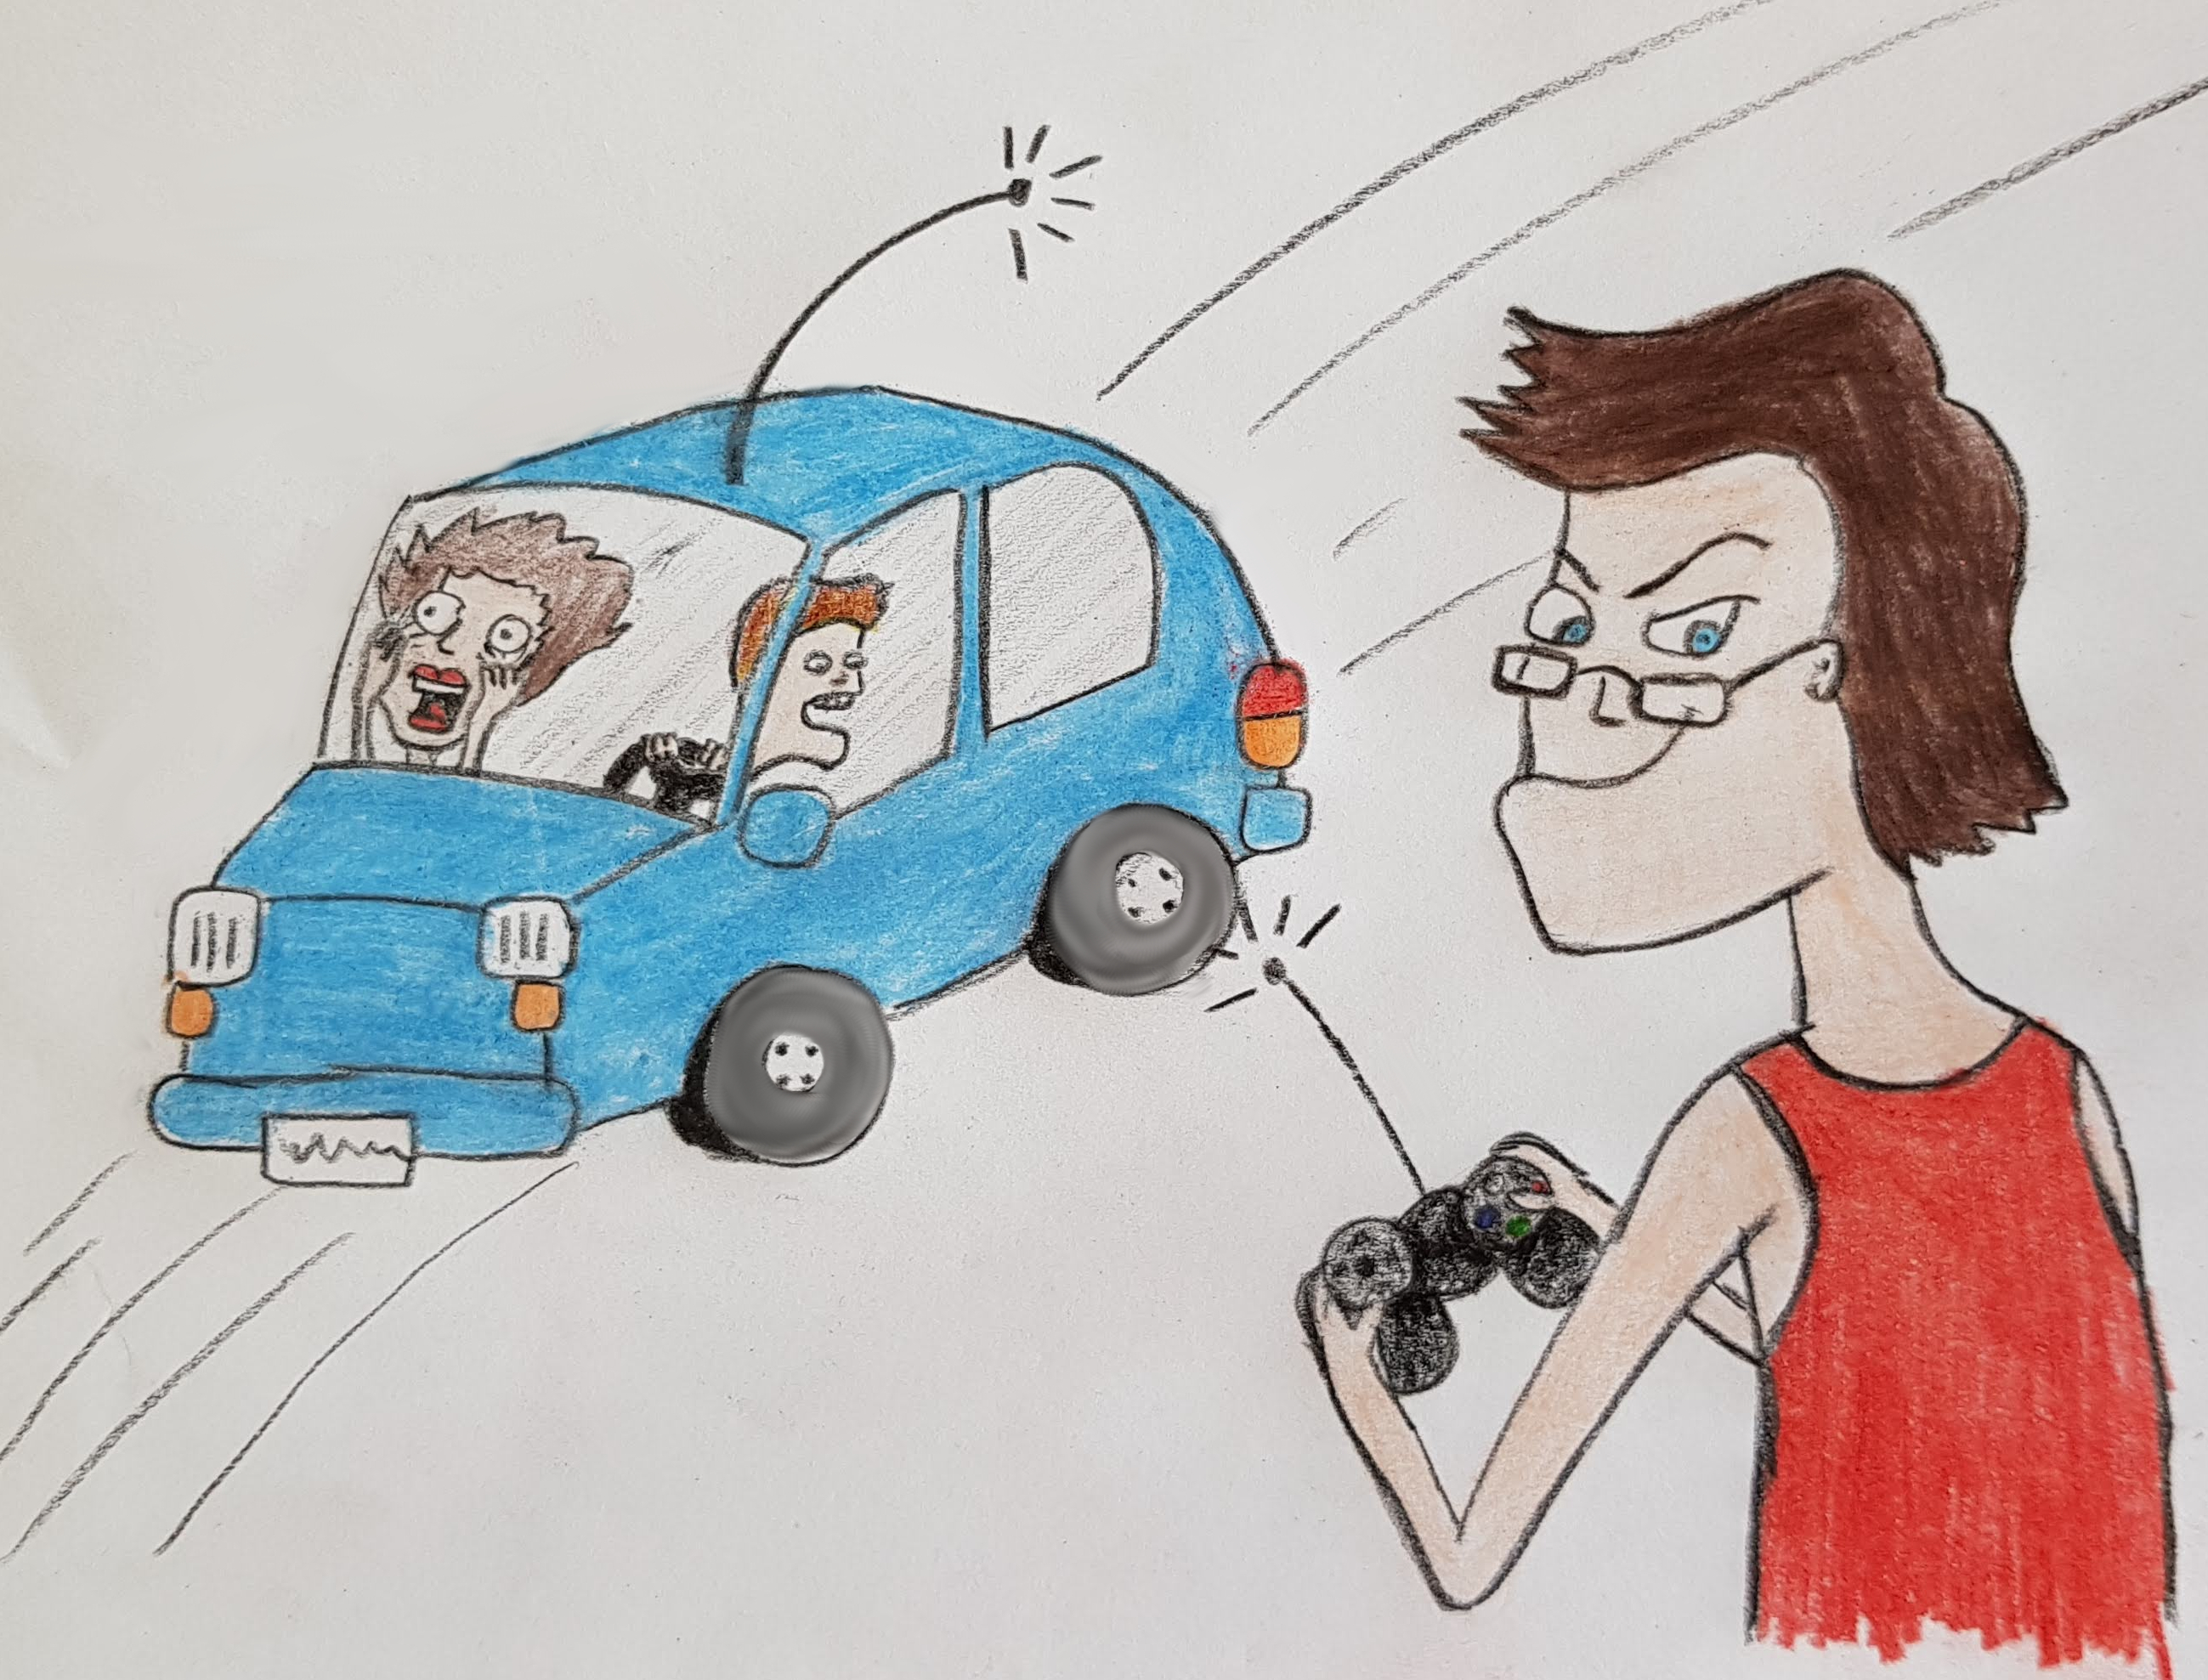
\includegraphics[width=1\linewidth]{Auto.jpg}
\end{figure}
\end{frame}

%------------------------------------------------

\begin{frame}
\begin{columns}[c]
\column{.65\textwidth}
\begin{itemize}
\item Kernel = Schl\"usselkomponente f\"ur sichere Systeme
\item Zugriffsteuerung auf Hardwarekomponenten
\item Fehler im Kernel kann die Sicherheit und Verl\"asslichkeit des kompletten Systems zum erliegen bringen.
\item Monolithische Designs: 
\begin{itemize}
\item Große Menge Code
\item Integration weiterer Funktionen.
\item Folge: Grundlegend schwach durch größere Anfällgkeit für Bugs.
\end{itemize}
\end{itemize}
\column{.35\textwidth}
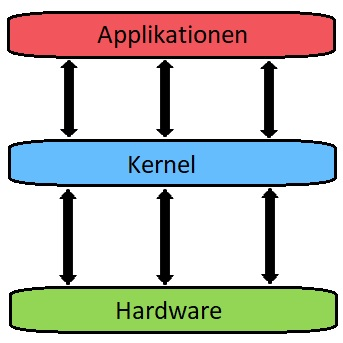
\includegraphics[width=0.8\linewidth]{Kernel.jpg}
\end{columns}
\begin{itemize}
\item Microkernel:\\
Konzentration auf die fundamentalen Funktionen eines Kernels: \\
z.B. Interprozesskommunikation, Scheduling, Speicherverwaltung
\item Durch Microkernels: Fehleranfälligkeit verringern (weniger Code $\Rightarrow$ Fehlerfreiheit formell verifizierbar)
\end{itemize}
\end{frame}

%------------------------------------------------
\section{seL4}
\begin{frame}
\frametitle{seL4}
\tikz[remember picture,overlay] 
   \node[anchor=north east,inner sep=0pt] 
    at([shift={(-1,-1.5)}]current page.north east){
\includegraphics[width=3cm]{sel4-logo.jpg}}; 
\begin{itemize}
\item In den 1990er Jahren entwickelt.
\item Basiert auf dem L4 Microkernel.
\item Stellt minimale Anzahl an services für Applikationen bereit. 
\end{itemize}
\end{frame}
%------------------------------------------------
\begin{frame}
\tikz[remember picture,overlay] 
   \node[anchor=north west,inner sep=0pt]
    at([shift={(1,-1)}]current page.north west) 		{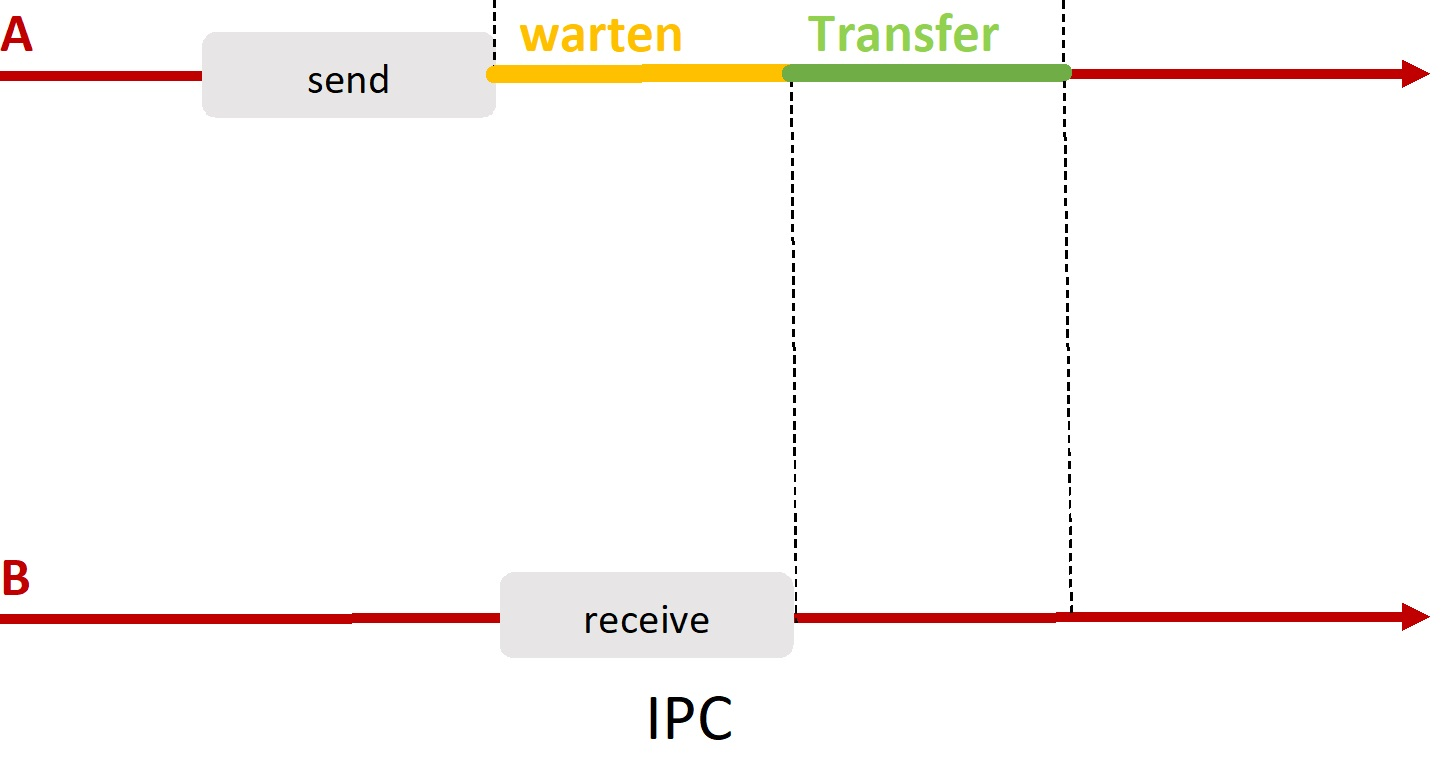
\includegraphics[width=5cm]{IPC2.jpg}};
\end{frame}
%------------------------------------------------
\begin{frame}
\tikz[remember picture,overlay] 
   \node[anchor=north west,inner sep=0pt]
    at([shift={(1,-1)}]current page.north west) 		{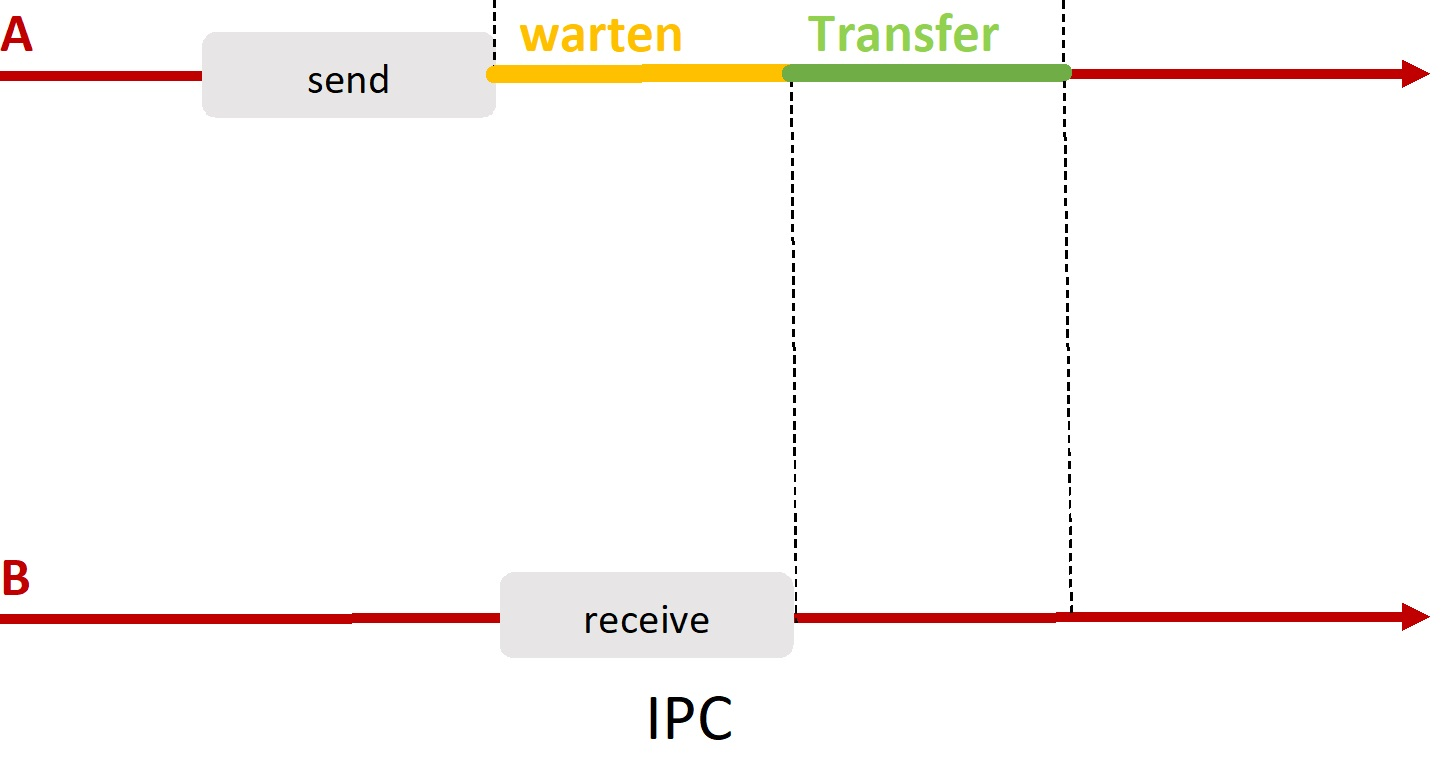
\includegraphics[width=5cm]{IPC2.jpg}};
\tikz[remember picture,overlay] 
   \node[anchor=south west,inner sep=0pt]
    at([shift={(1,1)}]current page.south west) 		{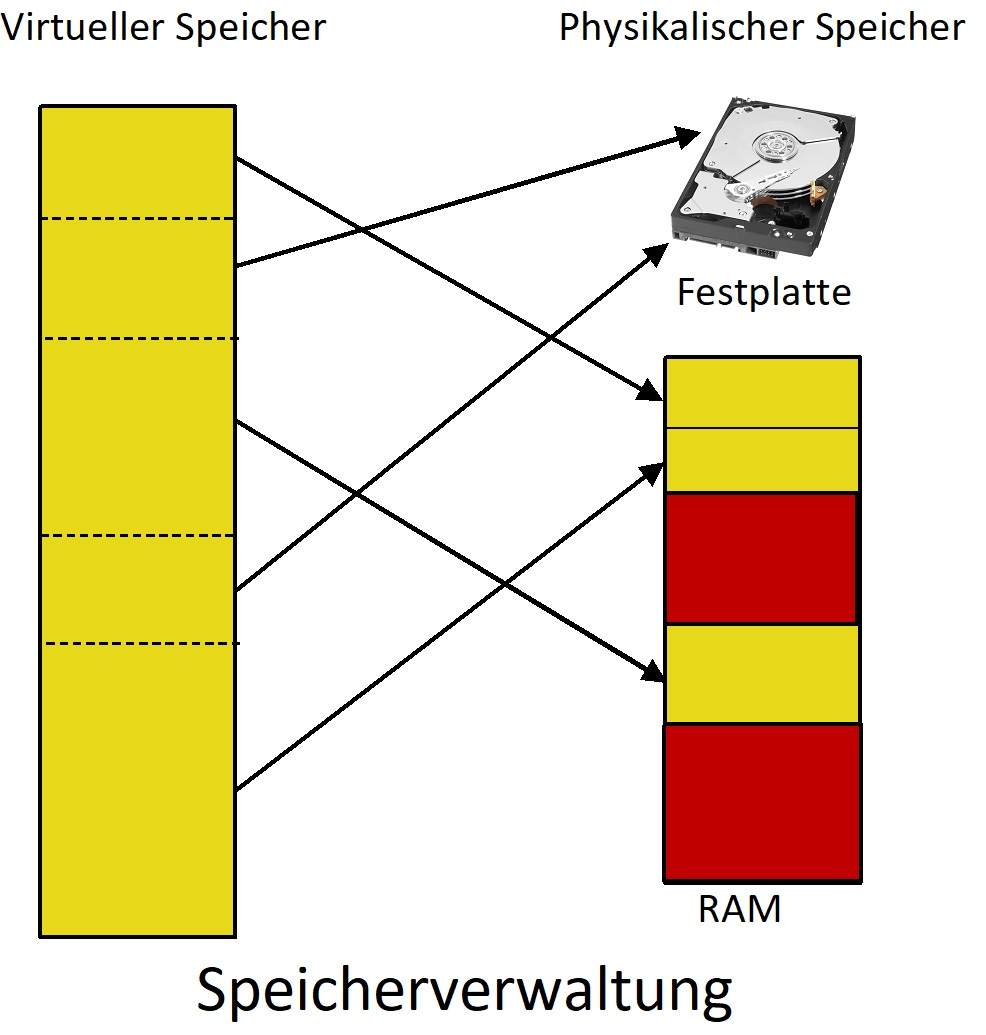
\includegraphics[width=4cm]{Speicher.jpg}};
\end{frame}
%------------------------------------------------
\begin{frame}
\tikz[remember picture,overlay] 
   \node[anchor=north west,inner sep=0pt]
    at([shift={(1,-1)}]current page.north west) 		{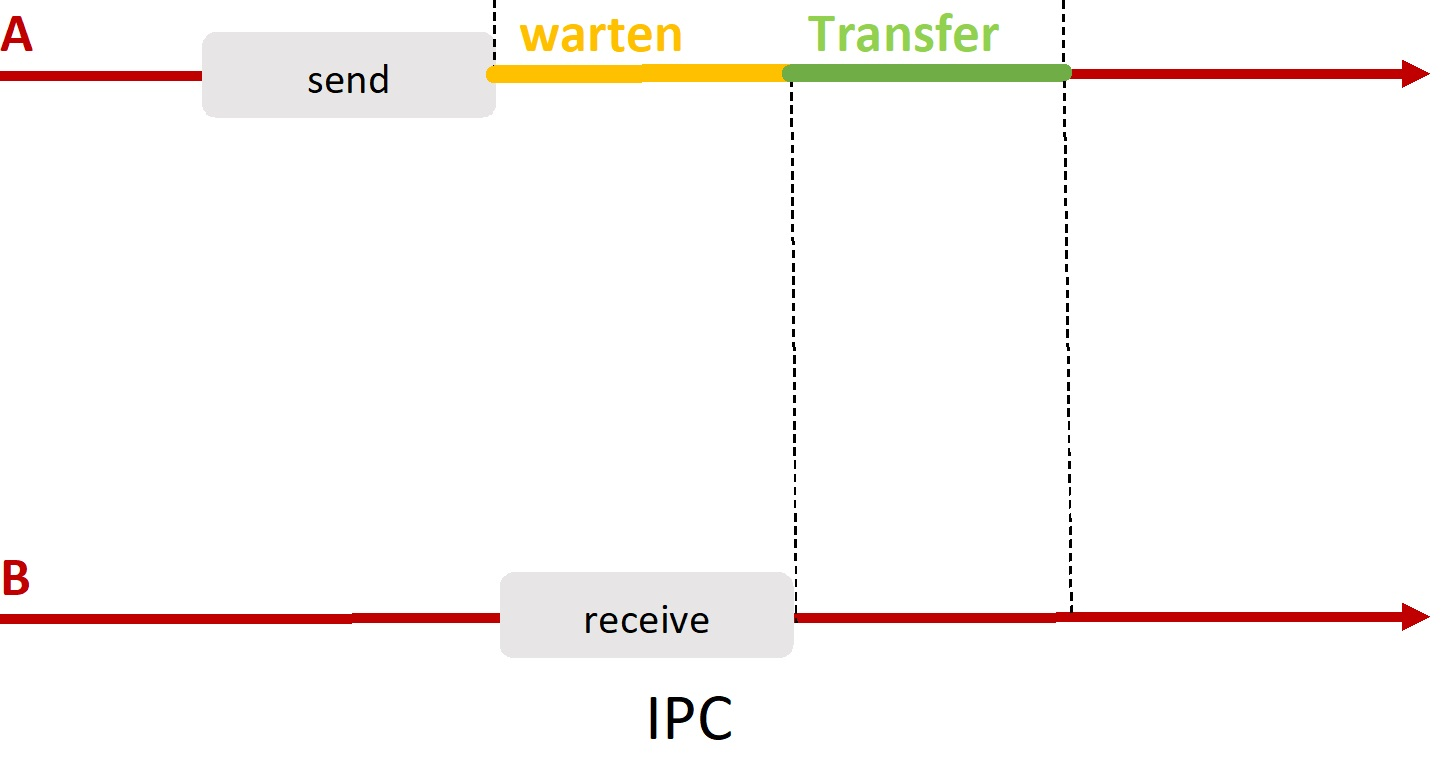
\includegraphics[width=5cm]{IPC2.jpg}};
\tikz[remember picture,overlay] 
   \node[anchor=south west,inner sep=0pt]
    at([shift={(1,1)}]current page.south west) 		{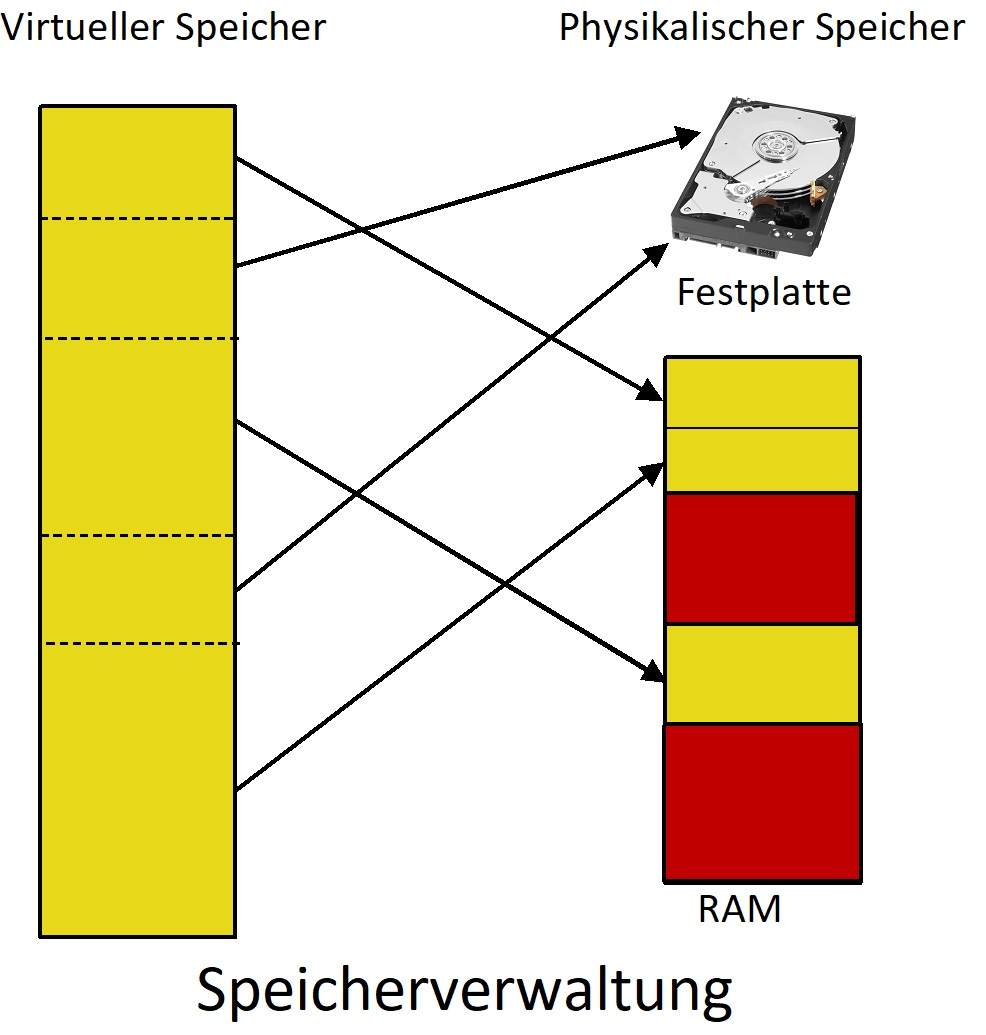
\includegraphics[width=4cm]{Speicher.jpg}};
    \tikz[remember picture,overlay] 
   \node[anchor=north east,inner sep=0pt]
    at([shift={(-1.5,-1)}]current page.north east) 		{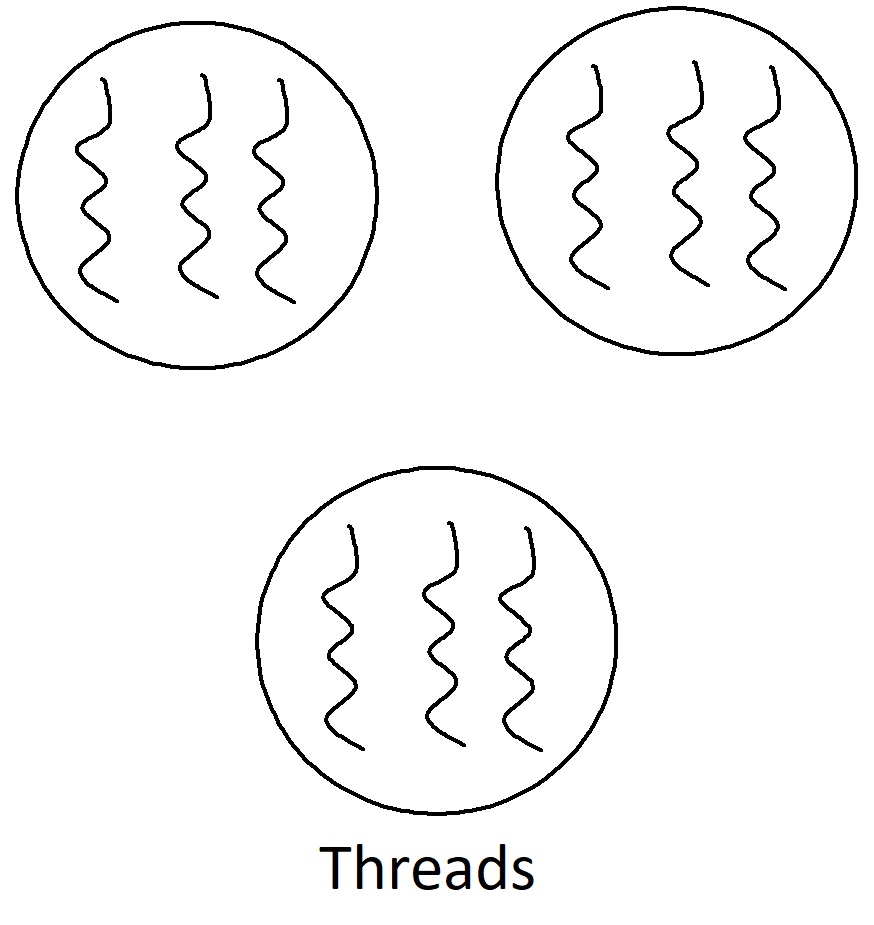
\includegraphics[width=3.5cm]{Threads.jpg}};
\end{frame}
%------------------------------------------------
\begin{frame}
\tikz[remember picture,overlay] 
   \node[anchor=north west,inner sep=0pt]
    at([shift={(1,-1)}]current page.north west) 		{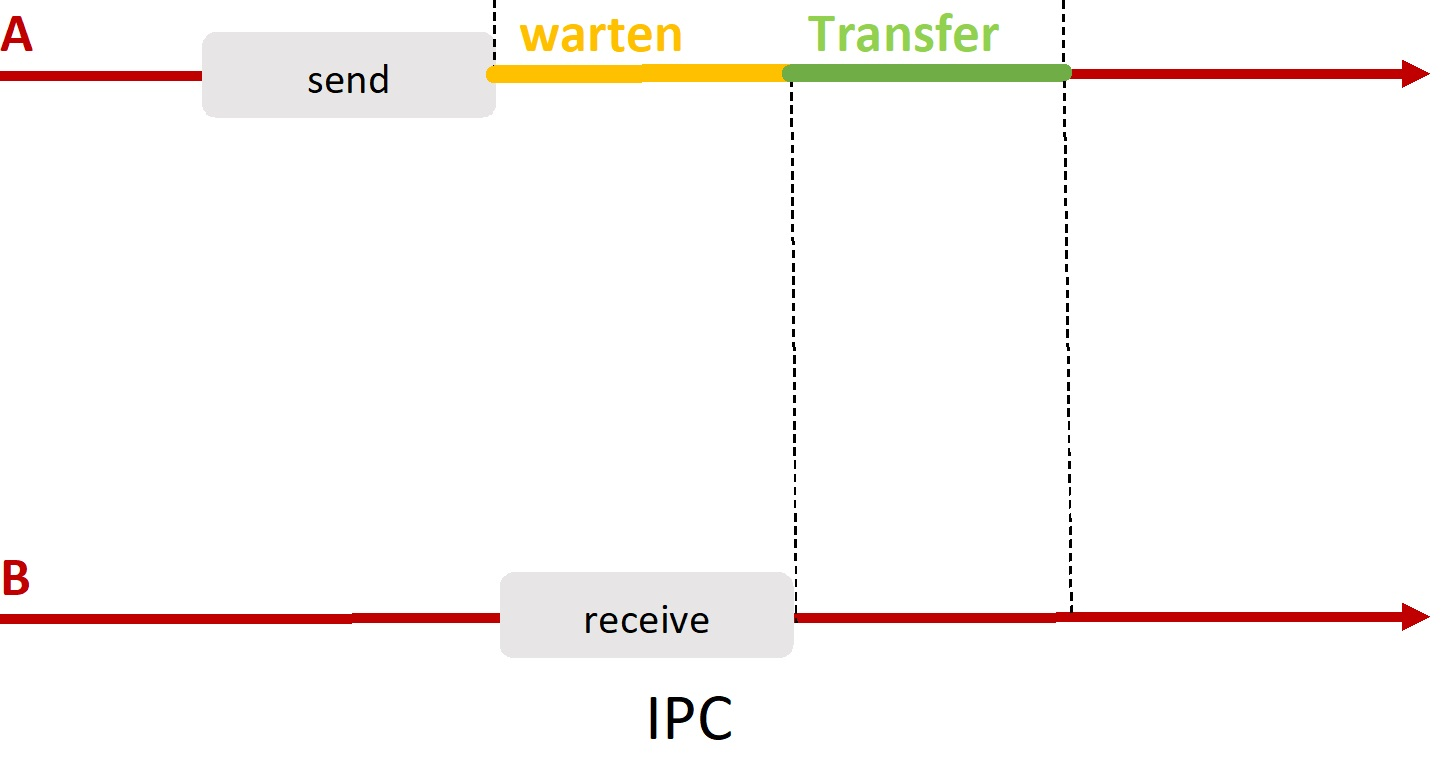
\includegraphics[width=5cm]{IPC2.jpg}};
\tikz[remember picture,overlay] 
   \node[anchor=south west,inner sep=0pt]
    at([shift={(1,1)}]current page.south west) 		{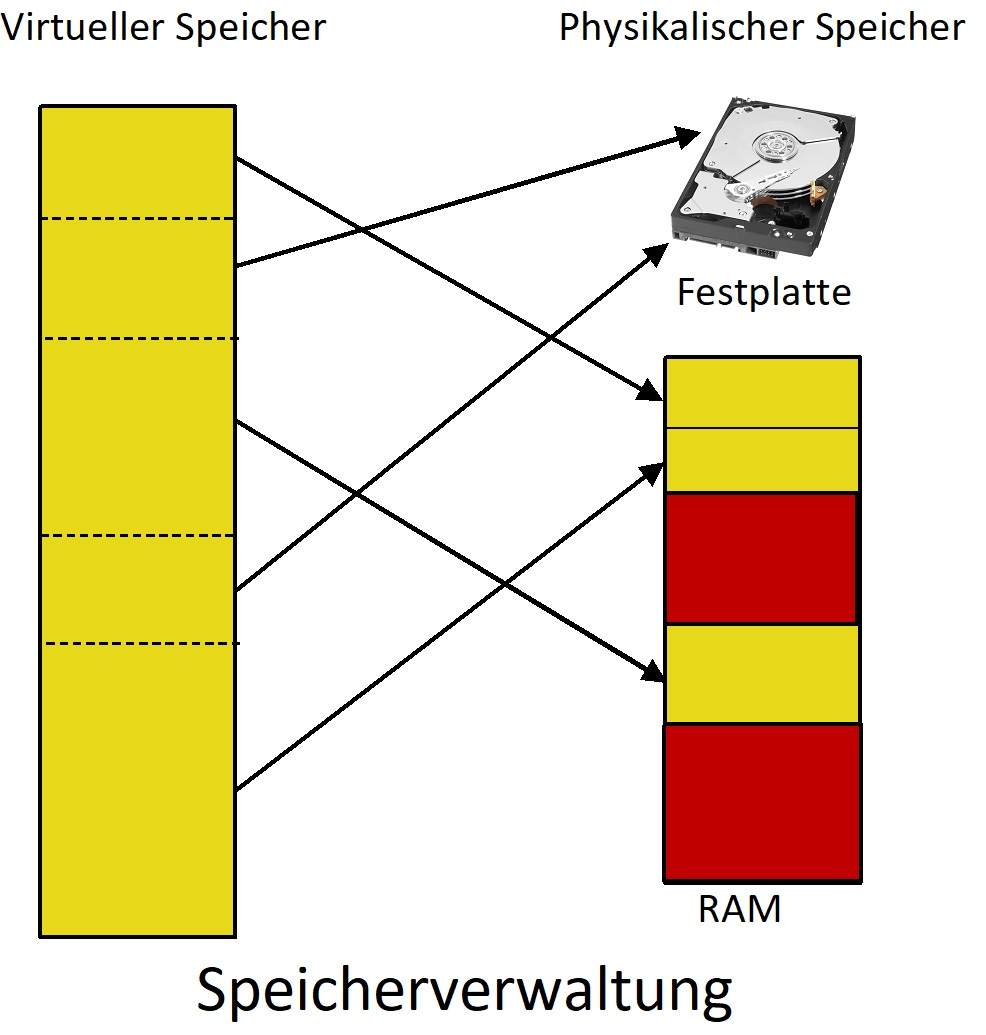
\includegraphics[width=4cm]{Speicher.jpg}};
    \tikz[remember picture,overlay] 
   \node[anchor=north east,inner sep=0pt]
    at([shift={(-1.5,-1)}]current page.north east) 		{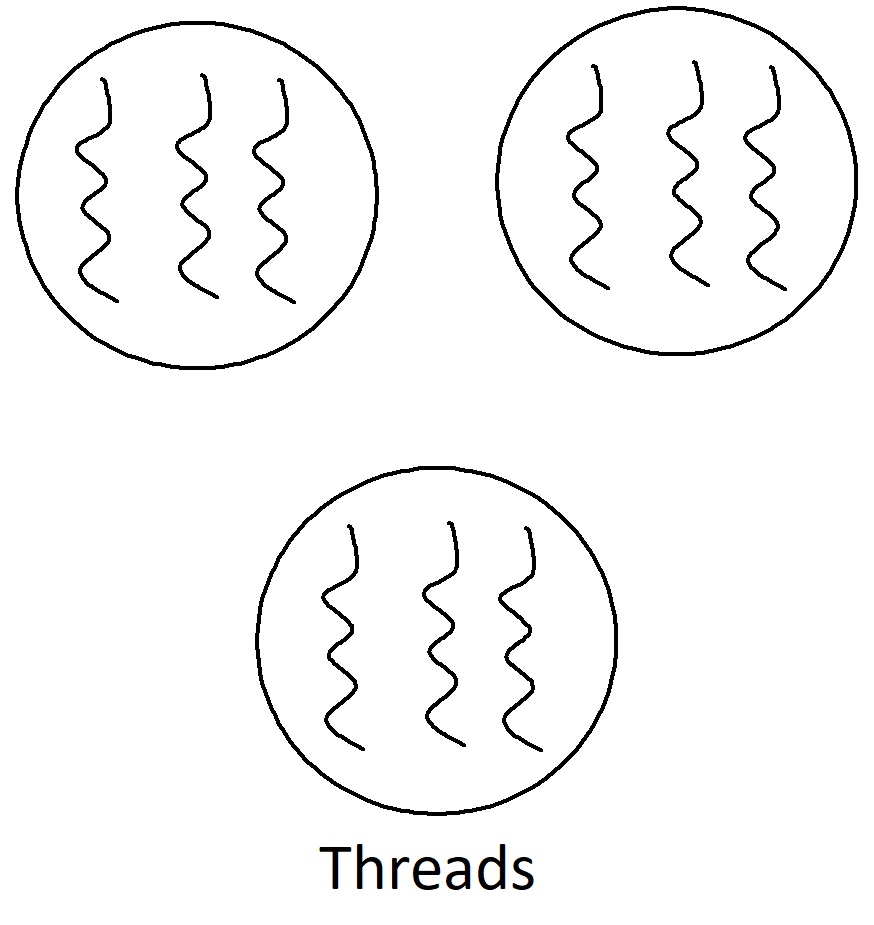
\includegraphics[width=3.5cm]{Threads.jpg}};
    \tikz[remember picture,overlay] 
   \node[anchor=south east,inner sep=0pt]
    at([shift={(-0.5,1)}]current page.south east) 		{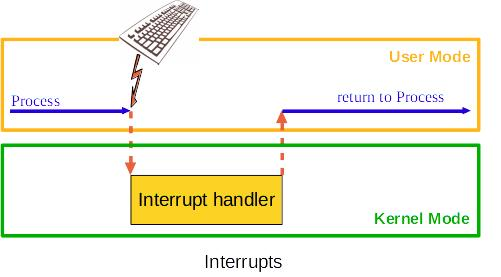
\includegraphics[width=6.5cm]{Interrupts.jpg}};
\end{frame}
%------------------------------------------------
\begin{frame}
\tikz[remember picture,overlay] 
   \node[anchor=north east,inner sep=0pt] 
    at([shift={(-1,-1.5)}]current page.north east){
\includegraphics[width=3cm]{sel4-logo.jpg}}; 
\begin{itemize}
\item In den 1990er Jahren entwickelt.
\item Basiert auf dem L4 Microkernel.
\item Stellt minimale Anzahl an services für Applikationen bereit. 
\item \textbf{Objekte:} implementieren jeweils die Abstraktion eines Services.
\end{itemize}
\end{frame}
%------------------------------------------------
\begin{frame}
\tikz[remember picture,overlay] 
   \node[anchor=north east,inner sep=0pt] 
    at([shift={(-1,-1.5)}]current page.north east){
\includegraphics[width=3cm]{sel4-logo.jpg}}; 
\begin{itemize}
\item In den 1990er Jahren entwickelt.
\item Basiert auf dem L4 Microkernel.
\item Stellt minimale Anzahl an services für Applikationen bereit. 
\item \textbf{Objekte:} implementieren jeweils die Abstraktion eines Services.
\item \textbf{Capabilities:} von Applikationen benötigt, um einen Service zu nutzen. 
\end{itemize}
\end{frame}
%------------------------------------------------
\begin{frame}
\tikz[remember picture,overlay] 
   \node[anchor=north east,inner sep=0pt] 
    at([shift={(-1,-1.5)}]current page.north east){
\includegraphics[width=3cm]{sel4-logo.jpg}}; 
\begin{itemize}
\item In den 1990er Jahren entwickelt.
\item Basiert auf dem L4 Microkernel.
\item Stellt minimale Anzahl an services für Applikationen bereit. 
\item \textbf{Objekte:} implementieren jeweils die Abstraktion eines Services.
\item \textbf{Capabilities:} von Applikationen benötigt, um einen Service zu nutzen. 
\item Die Rechte \texttt{Read, Write, Grant} und \texttt{Create} können in den Capabilities enthalten sein. 
\end{itemize}
\end{frame}
%------------------------------------------------
\begin{frame}
\begin{figure}[c]
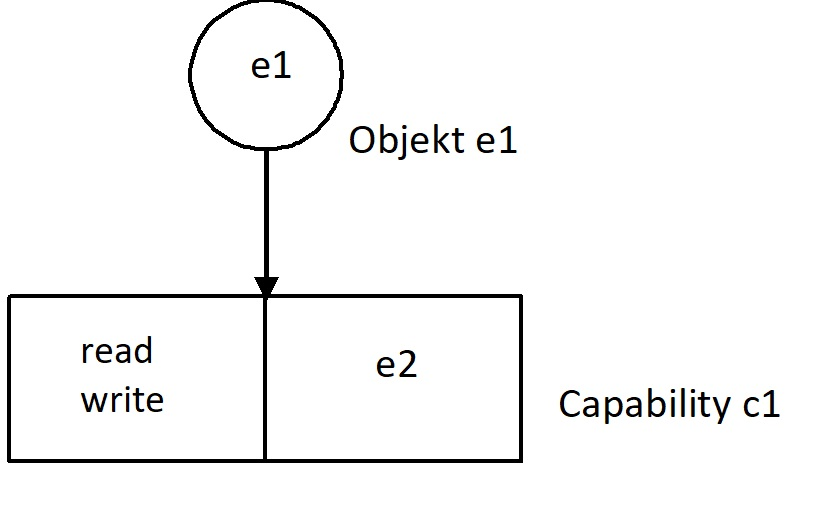
\includegraphics[width=4.5cm]{Capabilities1.jpg}
\end{figure}
\end{frame}
%------------------------------------------------
\begin{frame}
\begin{figure}[c]
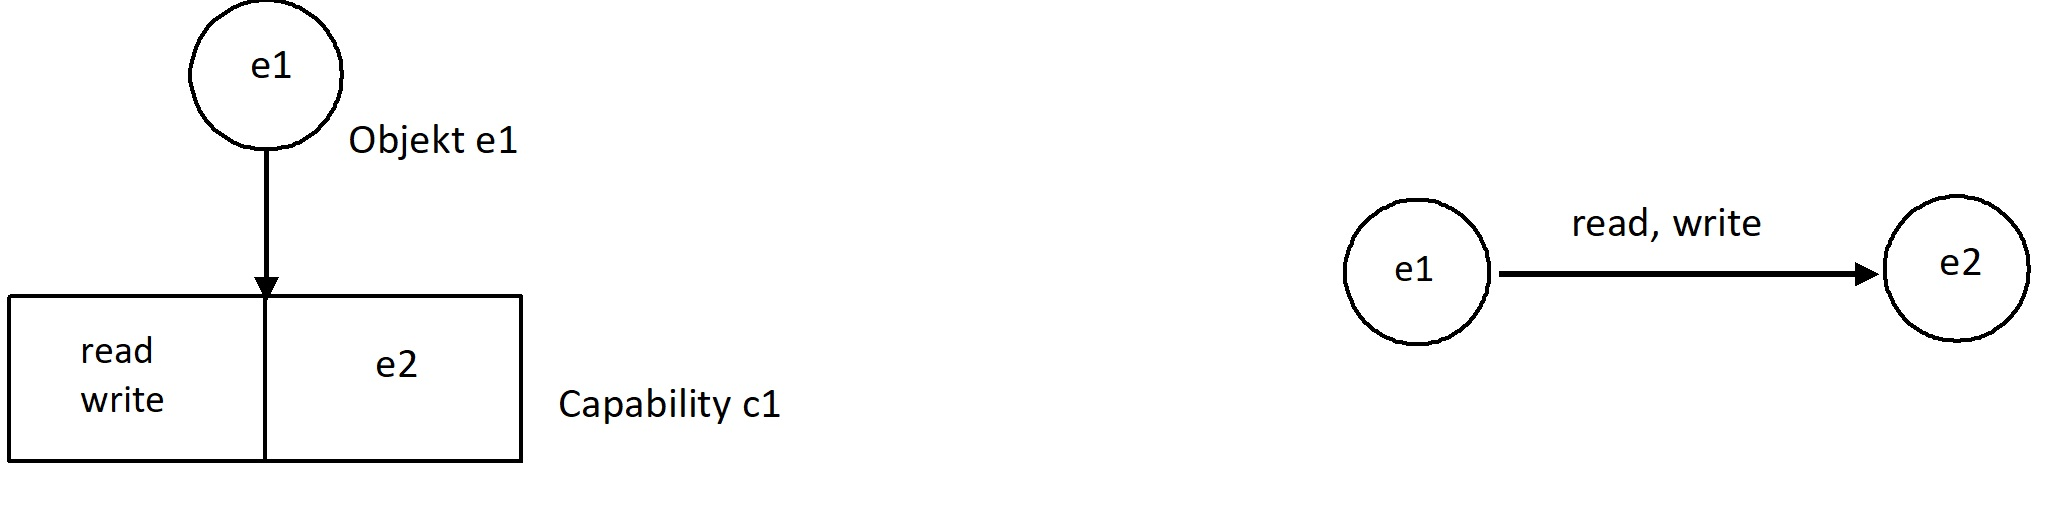
\includegraphics[width=10cm]{Capabilities2.jpg}
\end{figure}
\end{frame}
%------------------------------------------------
\begin{frame}
\subsection{Kernel Objekte}
\frametitle{Kernel Objekte}
\begin{itemize}
\item CNodes
\item IPC Endpoints
\item TCB
\item Virtual Memory
\item Interrupt Objects
\item Untyped Memory
\end{itemize}
\end{frame}
%------------------------------------------------
\begin{frame}
\frametitle{CNodes}
\begin{columns}[c]
\column{.65\textwidth}
\begin{itemize}
\item Lagern die Capabilities
\item Erhalten feste Zahl an Slots
\item Kernel konstruiert einen CDT (Capability Derivation Tree) zur Dokumentation der erstellten Capabilities und ihrer Verbindungen.
\item Mehrere CNodes bilden eine CSpace.
\end{itemize}
\column{.35\textwidth}
\tikz[remember picture,overlay] 
   \node[anchor=north east,inner sep=0pt] 
    at([shift={(-1,-1.5)}]current page.north east){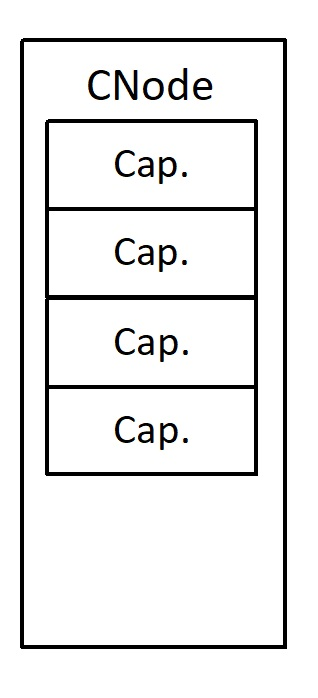
\includegraphics[width=1.5cm]{CNode.jpg}}; 
\tikz[remember picture,overlay] 
   \node[anchor=south east,inner sep=0pt] 
    at([shift={(-2,1.5)}]current page.south east){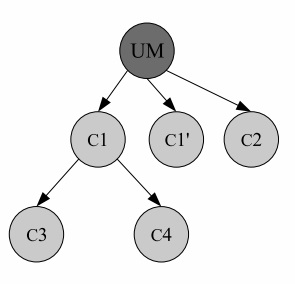
\includegraphics[width=3cm]{CDT.jpg}}; 
\end{columns} 
\end{frame}
%------------------------------------------------
\begin{frame}
\frametitle{IPC Endpoints}
\tikz[remember picture,overlay] 
   \node[anchor=north east,inner sep=0pt] 
    at([shift={(-1.5,-1.5)}]current page.north east){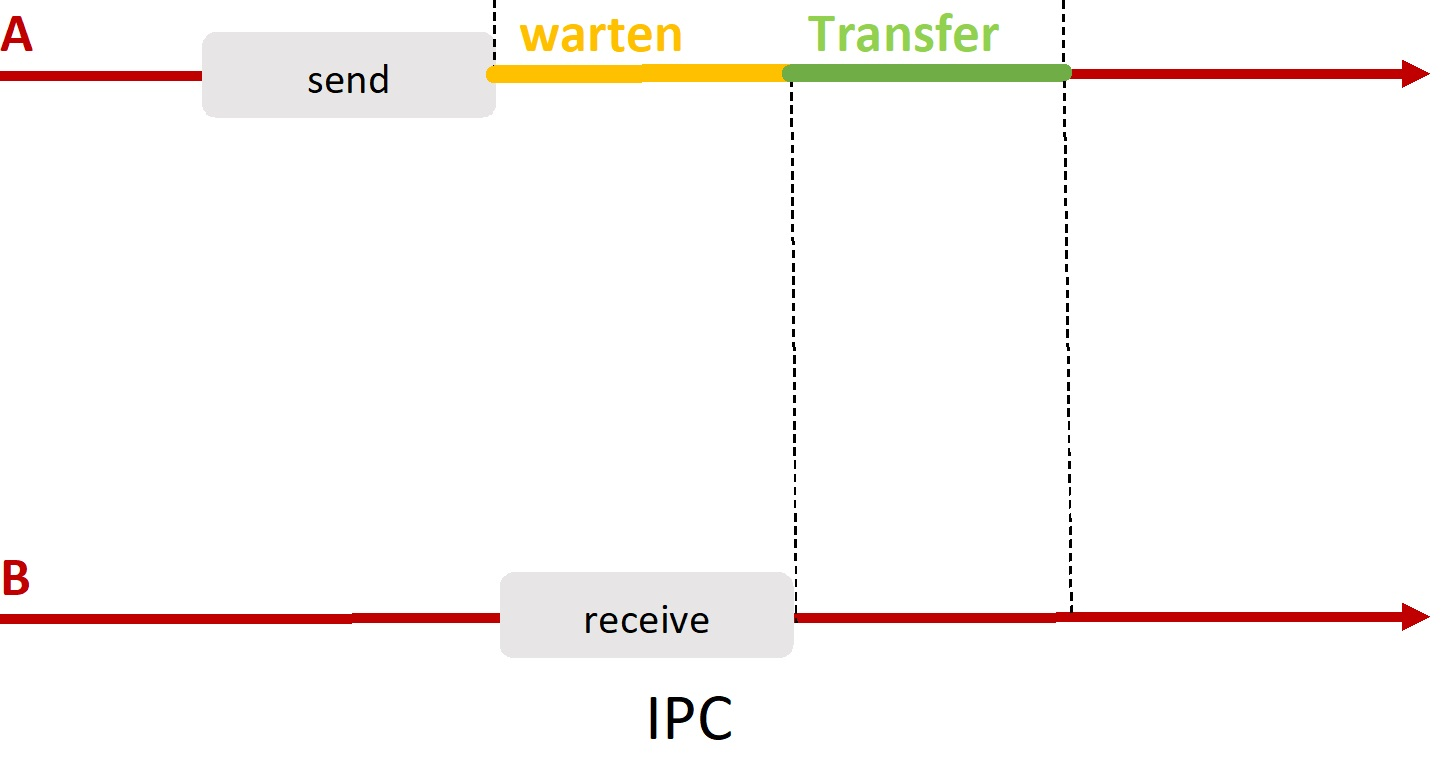
\includegraphics[width=4cm]{IPC2.jpg}}; 
\begin{itemize}
\item Notwendig für die Interprocesskommunikation
\item Unterscheidung: synchrone (SEP) und asynchrone (AEP) endpoints
\item Unterteilung der Threads in security domains
\item Kommunikation zwischen Threads aus verschiedenen security domains: nur über AEP
\item Generelle Einschränkung von Capabilities auf Endpoints zu \texttt{read} oder \texttt{write} only ist möglich.
\end{itemize}
\end{frame}
%------------------------------------------------
\begin{frame}
\frametitle{TCB}
\tikz[remember picture,overlay] 
   \node[anchor=north east,inner sep=0pt] 
    at([shift={(-1.5,-1.5)}]current page.north east){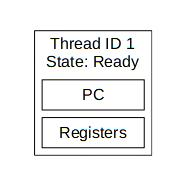
\includegraphics[width=3cm]{TCB.jpg}}; 
\begin{itemize}
\item \textit{Thread control block}
\item Repräsentiert einen Thread
\item Immer verknüpft mit einer CSpace und einer VSpace.
\end{itemize}
\end{frame}
%------------------------------------------------
\begin{frame}
\frametitle{Virtual Memory}
\tikz[remember picture,overlay] 
   \node[anchor=north east,inner sep=0pt] 
    at([shift={(-0.4,-1.5)}]current page.north east){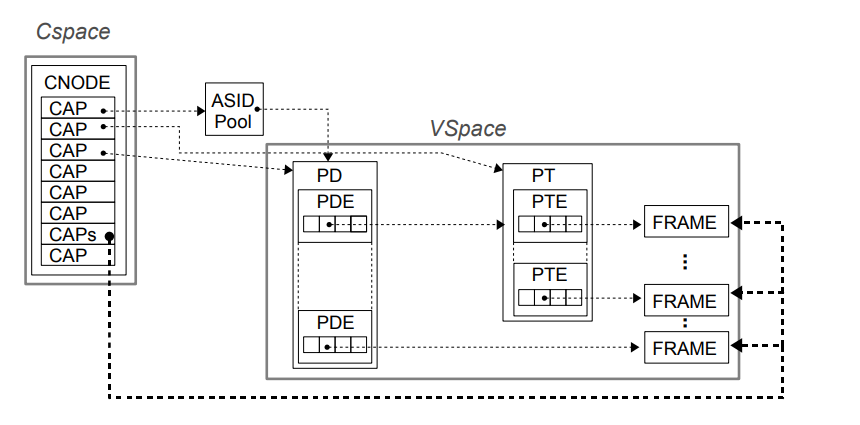
\includegraphics[width=5.5cm]{applicationIntern.png}};
\begin{itemize}
\item VSpache (Virtual adress space) \\ Verwaltung von virtuellem Speicher.
\item ASID Table:
\begin{itemize}
\item Globale Tabelle, feste Größe
\item Beim booten erstellt.
\item Dient zur Zuordnung von Mapping zu Adressräumen.
\end{itemize}
\item PageDirectory (PD)
\begin{itemize}
\item Oberes Level der 2-Level Page Tablestruktur. 
\item Enthält PDEs (page directory entries)
\end{itemize}
\end{itemize} 
\end{frame}
%------------------------------------------------
\begin{frame}
\begin{itemize}
\item PageTable (PT)
\begin{itemize}
\item 2. Level der 2-Level Page Tablestruktur.
\item Enthält PTEs (page table entries)
\item Ein PTE kann einen Pointer auf eine \texttt{Page} enthalten.
\end{itemize}
\item Page
\begin{itemize}
\item Abschnitt von physikalischem Speicher
\item Implementiert eine Seite im virtellen Speicher der VSpace.
\end{itemize}
\end{itemize}
\end{frame}
%------------------------------------------------
\begin{frame}
\frametitle{Interrupt Objects}
\tikz[remember picture,overlay] 
   \node[anchor=north east,inner sep=0pt]
    at([shift={(-0.5,-2)}]current page.north east) 		{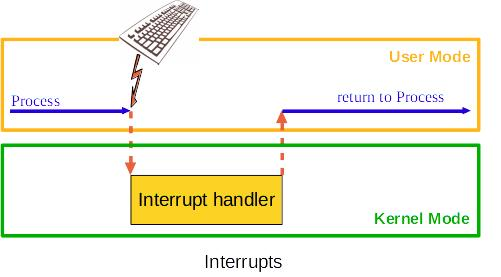
\includegraphics[width=4.5cm]{Interrupts.jpg}};
\begin{itemize}
\item Geben Applikationen die Möglichkeit \\Unterbrechungen von Hardwarekom-\\ponenten zu erhalten und zu bestätigen.
\item Eine InterruptHandler Capability erlaubt das Management einer Interruptursache. 
\item Eine InterruptController Capability erlaubt das Erstellen einer InterruptHandler Capability.  
\end{itemize}
\end{frame}
%------------------------------------------------
\begin{frame}
\frametitle{Untyped Memory Objects (UMO}
\tikz[remember picture,overlay] 
   \node[anchor=north ,inner sep=0pt]
    at([shift={(0,-2)}]current page.north) 		{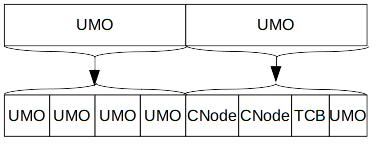
\includegraphics[width=4.5cm]{UMO.jpg}};
\begin{itemize}
\item Kapseln eine Region physikalischen Speichers ein.
\item Können in eine Gruppe kleiner UMOs geteilt werden.
\item Können mit \texttt{Retype()} in andere Objekttypen umgewandelt werden.
\end{itemize}
\end{frame}
%------------------------------------------------
\subsection{Memory Allocation Model}
\begin{frame}
\frametitle{Memory Allocation Model}
\begin{itemize}
\item Speicher für Kernelobjekte wird nicht dynamisch erzeugt.
\item Feste Speicherregionen zur Selbstverwaltung.
\item Zur Erzeugung neuer Objekte: Capabilities auf UMOs nötig
\item Initial User Thread einer Applikation erhält verfügbaren Speicher durch Capabilities auf UMOs.
\item Durch fest zugewiesenen Speicher und Selbstverwaltung des zugewiesenen Speichers $\Rightarrow$ Isolation des physikalischen Speichers zwischen Applikationen.
\end{itemize}
\end{frame}
%------------------------------------------------
\section{Take-Grant Model}
\begin{frame}
\frametitle{The Take-Grant Model\\{\small Das klassische Modell}}
\begin{itemize}
\item Subjekte und Objekte = Knoten
\item Berechtigungen = Pfeile
\item Gerichteter Graph = System
\item Regeln zur Veränderung des Graphen = Verschiedene Systemoperationen zur Verteilung der Berechtigunen. 
\item Standardregeln: \textit{take, grant, create, remove}
\end{itemize}
\end{frame}
%------------------------------------------------
\begin{frame}
\begin{columns}[t]
\column{.5\textwidth}
\textbf{Take Regel}
\begin{itemize}
\item S,X,Y = 3 verschiedene Knoten im Graph 
\item $\alpha$ = Pfeil von X nach Y 
\item $\gamma$ = Pfeil von S nach X
\item "t" bezeichnet das \textit{take} Recht
\item t $\in \gamma$
\end{itemize}
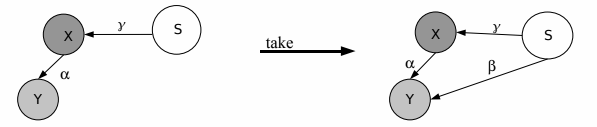
\includegraphics[width=6cm]{takeRule.png} \\
\textit{Take} fügt eine Kante von S nach Y, mit dem Lable $\beta \subseteq \alpha$ hinzu.
\column{.5\textwidth}
\textbf{Grant Regel}
\begin{itemize}
\item S,X,Y = 3 verschiedene Knoten im Graph 
\item $\alpha$ = Pfeil von S nach Y 
\item $\gamma$ = Pfeil von S nach X
\item "g" bezeichnet das \textit{grant} Recht
\item g $\in \gamma$
\end{itemize}
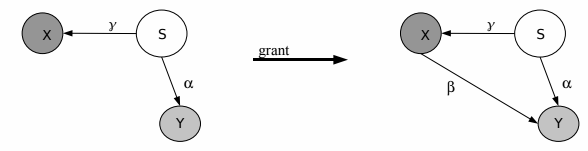
\includegraphics[width=6cm]{grantRule.png} \\
\textit{Grant} fügt eine Kante von X nach Y, mit dem Lable $\beta \subseteq \alpha$ hinzu.
\end{columns}
\end{frame}
%------------------------------------------------
\begin{frame}
\begin{columns}[t]
\column{.5\textwidth}
\textbf{Create Regel}\\
S = Knoten im Graph 
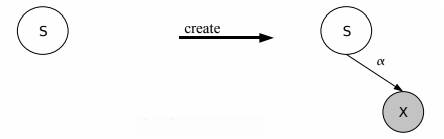
\includegraphics[width=5cm]{createRule.png} \\
\textit{Create} fügt einen neuen Knoten und eine Kante von S nach X, mit dem Lable $\alpha$ hinzu.
\column{.5\textwidth}
\textbf{Remove Regel}
\begin{itemize}
\item S,X = verschiedene Knoten im Graph 
\item $\alpha$ = Pfeil von S nach X 
\end{itemize}
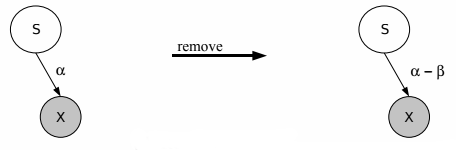
\includegraphics[width=6cm]{removeRule.png} \\
\textit{Remove} entfernt $\beta$ Lable von $\alpha$ oder den kompletten Pfeil, falls $\alpha - \beta = \lbrace\rbrace$
\end{columns}
\end{frame}
%------------------------------------------------
\begin{frame}
\frametitle{{\small Take-Grant für den seL4 verändert}}
Modifikationen:
\begin{itemize}
\item \textit{Create:} 
\begin{itemize}
\item Objekt das \textit{create} ausführt (e1), benötigt create Rechte in einer seiner Capabilities.
\item Neuer Knoten wird erstellt.
\item Objekt e1 kann anderem Objekt e2 alle verfügbaren Rechte auf das neue Objekt geben, wenn e1 \textit{grant} Rechte auf e2 besitzt.
\end{itemize}
\item \textit{Remove:} \\
Entfernt nicht mehr Teile eines Lables, sondern die komplette Capability. 
\item \textit{Revoke:} \\
Entfernt im CDT alle Capabilities ab einer angegebenen.
\item \textit{Grant} wurde nicht verändert und \textit{take} wurde entfernt.
\end{itemize}
\end{frame}
%------------------------------------------------
\begin{frame}
\begin{itemize}
\item Objekte u. Subjekte = \textit{entities}
\item Kopieren von Capabilities:
\begin{itemize}
\item \texttt{mint}: kopierte Capability = Kindknoten der originalen im CDT (weniger oder gleich viel Rechte wie das Original)
\item \texttt{imitate}: kopierte Capability = Geschwisterknoten der originalen im CDT (gleich viel Rechte wie das Original)
\end{itemize}
\item Isolation durch Subsysteme (durch \textit{grant} verbundene entities)
\end{itemize}
\end{frame}
%------------------------------------------------
\section{Noninterference}
\begin{frame}
\frametitle{Noninterference}
\begin{itemize}
\item Kontrolliert den Informationsfluss in einem System
\item Objekte aus unterschiedlichen Sicherheitslevels dürfen sich nicht gegenseitig beeinflussen.
\item Variablen im Model = L (low security) oder H (high security) Variablen.
\item Geoffrey Smith in \href{http://users.cis.fiu.edu/~smithg/papers/sif06.pdf}{%
"Principles of Secure Information Flow Analysis"}: \\
		\textbf{$\dq$Program c satisfies noninterference if, for any memories $\mu$ and $\nu$ that agree on L variables, the memories produced by running c on $\mu$ and on $\nu$ also agree on L variables (provided that both runs terminate successfully).$\dq$} 
\item Notation für die Noninterference policy: $\leadsto$
\item L$\leadsto$H $\equiv$ Erlaubter Informationsfluss: von L nach H
\item $\mu$ und $\nu$ stimmen auf L Variablen überein, wenn sie eine Äquivalenzrelation $\mu$ $\overset{\text{L}}{\sim}$ $\nu$ erfüllen.
\end{itemize}
\end{frame}
%------------------------------------------------
\section{Formalisierung des Take-Grant Models}
\begin{frame}
	\frametitle{Formalisierung des Take-Grant Models}
	\begin{itemize}
		\item Entities werden Indentifieziert durch Speicheradresse (modelliert durch eine natürliche Zahl):\\ 
				\textbf{type$\_$synonym} \texttt{ entity$\_$id = nat}
		\item \textit{Zugriffsrechte} \\
		\textbf{datatype} \texttt{ rights = Read | Write | Grant | Create}
		\item \textit{Capabilities} \\
		\textbf{record} 
		\texttt{	
			\begin{tabular}[t]{ll}
				cap = & entity :: entity$\_$id \\
				& rights :: rights set
			\end{tabular}}
		\item \textit{Entities} \\
		\textbf{record } \texttt{ 						
			entity = caps :: cap set}
		\item \textit{Status (state) des Systems} \\
		\textbf{record}
		\texttt{
			\begin{tabular}[t]{ll}
				state =	& heap :: entity$\_$id $\Rightarrow$ entity \\
				& next$\_$id :: entity$\_$id
			\end{tabular}}
	\end{itemize}
\end{frame}
%------------------------------------------------
\begin{frame}
	\begin{itemize}
		\item \textit{Verschiedene Systemoperartionen} \\
			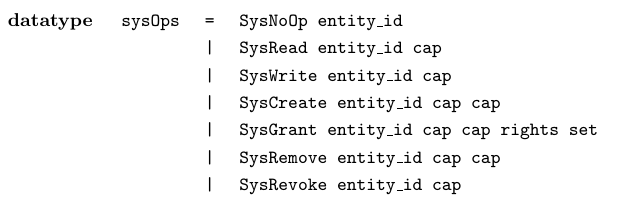
\includegraphics[width=6cm]{Sysops.png}
		\item \textit{legal} prüft ob eine Systemoperation legal ist.
			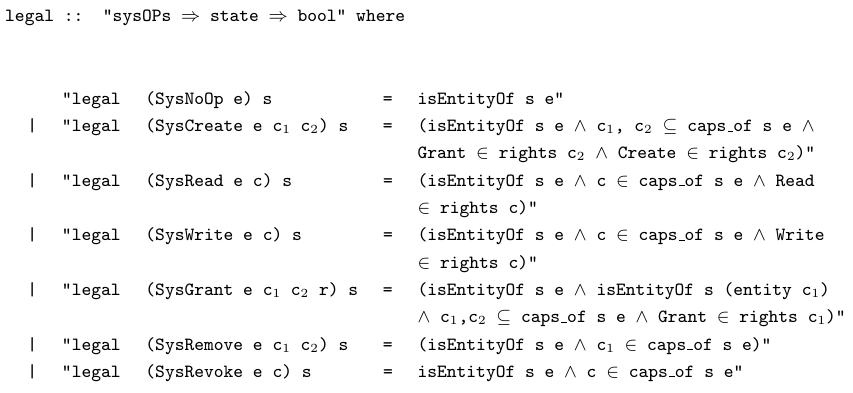
\includegraphics[width=8cm]{legal.png}
	\end{itemize}
\end{frame}
%------------------------------------------------
%----------------------------------------------------------------------------------------

\end{document} 
